% Architecture figure for Ch15 ("MCP: Designing External Capability").
% Standalone TikZ; compiled by `book-scaffold build-figures` via pdflatex -> pdftocairo -> SVG.
% MCP host/client/server split with capability negotiation and the three primitives
% (tools = model-controlled, resources = app-driven, prompts = user-controlled).
% NOTE: no TikZ style named 'cap', 'coord', 'axis', or 'sub' (they collide with built-ins).
\documentclass[tikz,border=4mm]{standalone}
\usepackage{tikz}
\usetikzlibrary{positioning, arrows.meta, calc, fit, backgrounds}

\begin{document}
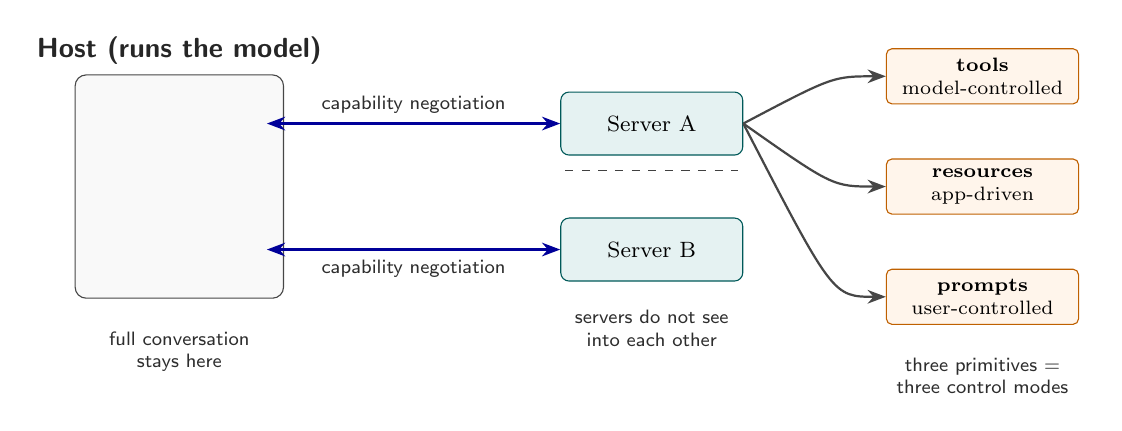
\begin{tikzpicture}[
  font=\sffamily,
  hostbox/.style={draw=gray!55!black, fill=gray!5, rounded corners=4pt, align=center,
    inner sep=6pt, font=\footnotesize\bfseries},
  clientbox/.style={draw=blue!70!black, fill=blue!8, rounded corners=3pt, align=center,
    text width=2.0cm, minimum height=0.8cm, inner sep=3pt, font=\footnotesize},
  serverbox/.style={draw=teal!70!black, fill=teal!10, rounded corners=3pt, align=center,
    text width=2.1cm, minimum height=0.8cm, inner sep=3pt, font=\footnotesize},
  primbox/.style={draw=orange!75!black, fill=orange!8, rounded corners=2pt, align=center,
    text width=2.3cm, minimum height=0.7cm, inner sep=2pt, font=\scriptsize},
  link/.style={-Stealth, thick, draw=gray!55!black},
  neg/.style={Stealth-Stealth, thick, draw=blue!60!black},
  lbl/.style={font=\sffamily\scriptsize, text=gray!35!black}
]

% --- Host (left): runs the model + multiple clients ---
\node[clientbox] (c1) at (0,0)    {client A};
\node[clientbox] (c2) at (0,-1.6) {client B};
\node[hostbox, fit=(c1)(c2), label={[font=\sffamily\bfseries,text=gray!30!black]above:Host (runs the model)}] (host) {};
\node[lbl, text width=2.4cm, align=center] at (0,-2.9)
  {full conversation\\stays here};

% --- Servers (right): one per client, 1:1 ---
\node[serverbox] (s1) at (6.0,0)    {Server A};
\node[serverbox] (s2) at (6.0,-1.6) {Server B};

% client-server 1:1 links with capability negotiation
\draw[neg] (c1) -- node[lbl, above]{capability negotiation} (s1);
\draw[neg] (c2) -- node[lbl, below]{capability negotiation} (s2);

% isolation note between servers
\draw[dashed, draw=gray!50!black] (4.9,-0.6) -- (7.1,-0.6);
\node[lbl, text width=2.4cm, align=center] at (6.0,-2.6)
  {servers do not see\\into each other};

% --- The three primitives exposed by a server ---
\node[primbox] (p1) at (10.2,0.6)  {\textbf{tools}\\model-controlled};
\node[primbox] (p2) at (10.2,-0.8) {\textbf{resources}\\app-driven};
\node[primbox] (p3) at (10.2,-2.2) {\textbf{prompts}\\user-controlled};

\draw[link] (s1.east) .. controls (8.3,0.6) .. (p1.west);
\draw[link] (s1.east) .. controls (8.3,-0.8) .. (p2.west);
\draw[link] (s1.east) .. controls (8.3,-2.2) .. (p3.west);

\node[lbl, text width=2.6cm, align=center] at (10.2,-3.2)
  {three primitives =\\three control modes};

\end{tikzpicture}
\end{document}
